\documentclass[12pt]{report}

\usepackage{url}
%\usepackage[dvips]{graphicx}
\usepackage{graphicx}
\usepackage{amsmath}
\usepackage{longtable}
\usepackage{amssymb}
\usepackage[round]{natbib}
\bibpunct{(}{)}{;}{a}{,}{,}
\usepackage{cite}
\usepackage{longtable}
\usepackage{dcolumn}
\usepackage{booktabs}

% If there are any other \usepackage commands, put them here.

\usepackage{guthesis} % Must be the last package

\newtheorem{theorem}{Theorem}[section]
\newenvironment{proof}[0]{\textit{Proof.}}{}
\newcommand{\qed}{\hfill $\Box$}

% To comment out multiple lines of text.
\long\def\comment#1{}

\title{The Effect of Electronic Healthcare Record Adoption
on Patient-specific Health Education Prescription, Time Utilization, and Returned Appointments: A Propensity Score Weighted Analysis}

\author{Huade Huo}

\previousdegree{B.Mg.}

\thisdegree{Master of Public Policy}  % or Doctor of Philosophy, etc.

\thisdiscipline{Public Policy}

\thesistype{Thesis}     % or Dissertation

% defense or approval date, not today's date...
\thesisday{11}
\thesismonth{April}
\thesisyear{2015}

\professor{Yuriy Pylypchuk}
%\secondprofessor{Alonzo Church}   % Only if you have 2 major professors!

\fulltitle{The Effect of Electronic Healthcare Record Adoption
on Patient-specific Health Education Prescription, Time Utilization, and Returned Appointments: A Propensity Score Weighted Analysis}

\indexwords{Electronic~Healthcare~Record, Patient-specific Health Education, Time Utilization,
            Returned Appointments, Propensity Score Weighting, Theses~(academic)}

\begin{document}

\pagenumbering{roman}

\maketitle    % Creates title page, copyright page if any, and approval page.

\begin{abstract}
This is the abstract, a brief summary of the contents of the entire thesis.
It is limited to 350 words.

The abstract page(s) are not numbered and are not necessarily included
in the bound copies.  Likewise, the signature page is not counted in
page numbering because not all copies contain it.

Throughout this sample thesis, {\bf please note
that the layout obtained with \LaTeX\ is not meant to be a
perfect duplicate of the Microsoft Word examples in the \emph{Graduate
School Style Manual.}}  \LaTeX\ has additional typographic tools at its
disposal, such as {\sc small capitals} and various subtle adjustments
of spacing, which are used by the Georgetown \LaTeX\ style sheet in
accordance with the standard practices of the book-printing industry.

The index words at the bottom of the abstract should be chosen carefully,
preferably with the help of one or two of your colleagues.
They are the words by which people will find your thesis when searching
the scientific literature.
If you want to get credit for your ideas, be sure to choose a good set of
index words so that people doing related work will know about yours.
\end{abstract}


\chapter*{Dedication}
The Dedication is optional, but if it is included, it should have
a roman numeral page number but not be included in the table of
contents.  To achieve that, we declare it as a \verb"\chapter*" in \LaTeX.


\pseudochapter{Acknowledgments}

In a real thesis, this section would contain acknowledgments such
as, ``This work was funded by National Science Foundation Grant
Number AAA-00-00000 (Benjamin Franklin, Principal Investigator),''
and ``I would like to thank John Doe for helping me proofread my
thesis and Mary Roe for drawing my graphs.''

The acknowledgments are included in the table of contents but do
not have a chapter number.  To achieve that, we
declare them to be a \verb"\pseudochapter" (which is defined only in
\verb"guthesis.sty").

I (Mark Maloof) would like to thank Michael Covington for developing
this \LaTeX\ style sheet for the University of Georgia.
Zachary Hunter deserves special thanks for revising the UGA style
file to work with the new version of \LaTeX\ (2e) as well as the
previous version (2.09).
The revisions in
Version 3.0 of \verb"guthesis.sty" are
largely the work of Isidor Ruderfer.
Other credits appear in the style sheet itself.


\tableofcontents

\listoffigures  % Optional - Omit this line if you don't want a list of figures.
\listoftables   % Optional - Omit this line if you don't want a list of tables.

\newpage

\pagenumbering{arabic}  % Ordinary pages have Arabic numerals.
\chapter{Introduction (working)}
The US spend 17.9\% of GDP on health expenditure in 2013, according to the World Bank, and it is continuing to growth. Some scholars proposed that one way to reduce health care spending and improve health care efficiency is to adopt the Electronic Healthcare Record (EHR). The Obama Administration has prioritized the improvement of quality and efficiency of the health care system. President Obama signed the American Recovery and Reinvestment Act of 2009 which provides financial incentive for adoption and meaningful use of electronic health records. The adoption of EHR increased rapidly [CITATION NEEDED].

Given the increasing adoption of EHR, and the implementation of EHR incentive programs, the effect of electronic health care record on health outcomes are of interest. Empirically measured effect of adopting EHR on cost is still very limited, and the results are mixed.

\chapter{Literature review}

\section{Background}

In 2009, the US Congress passed the American Recovery and Reinvestment Act (ARRA), which appropriates funds to promote the adoption and use of health information technology (HIT). The American Recovery and Reinvestment Act has set aside \$2 billion which will go towards programs developed by the National Coordinator and Secretary to help health care providers implement HIT and provide technical assistance through various regional centers \citep{hhs_recovery}.

The Centers for Medicare \& Medicaid Services launched the Medicare and Medicaid Electronic Health Care Record (EHR) Incentive Programs after the passage of ARRA in 2009. These programs provide incentive payments to eligible professionals, eligible hospitals, and critical access hospitals (CAHs) as they adopt, implement, upgrade or demonstrate meaningful use of certified EHR technology. In order to receive the EHR stimulus money, the HITECH act (ARRA) requires eligible physicians to show "meaningful use" of an EHR system.

Take the Medicare EHR incentive program as an example. Eligible physicians must attest yearly that they demonstrate meaningful use to receive the EHR incentive and avoid a Medicare payment adjustment. In order to demonstrate meaningful use in 2014 Stage 1, eligible professionals must meet 13 required core objectives and 5 menu objectives from a list of 9. The core objectives includes recording selected patient demographics, maintaining active medication lists, protecting electronic health information, etc. The menu objectives include using certified EHR technology to identify patient-specific education resources, sending patient reminders, and implementing drug formulary checks, etc. \citep{stage1}.

\section{Effect of EHR on health expenditure}

Limited empirical studies have estimated the potential net benefits that could arise from adopting health information technologies (HITs), including EHR at the national level. The RAND Corporation estimated that annual net savings to the health care sector from efficiencies alone could be \$77 billion or more based on surveys, publications, interviews, and an expert panel review \citep{Rand2005}. Hillestad et al. claimed that effective EHR implementation and networking could eventually save more than \$81 billion annually by improving health care efficiency and safety. Savings could be doubled by using health information technology to preventive care and chronic disease management \citep{Hillestad2005}. However, some other researchers do not find that the adoption of EHR has a positive cost saving effect on national health expenditure. For example, Adler-Milstein et al. found that ambulatory EHR adoption did not impact the total cost, although it slowed ambulatory cost growth \citep{Adler-Milstein2013}. Sidorov claimed that much of the literature on EHRs fails to support the primary rationales for using it, and it is unlikely that the U.S. health care bill will decline as a result of EHR alone \citep{Sidorov2006}. There are also researchers that suggest the adoption of EHR has a negative effect on cost-reduction  \citep{Teufel2012}.

EHR also provides a platform for predictive analysis, saving health care spending by allocating medical resources efficiently. Bates et al. proposed there are unprecedented opportunities to use big data, acquired from EHR, to reduce the costs of health care in the United States \citep{Bates2014}. Roski et al. also pointed out big data has the potential to create significant value in health care by improving outcomes while lowering costs \citep{Roski2014}. However, the integration of EHR into predictive analytics is still challenging. Roski et al. claimed that big data's success in creating value in the health care sector may require changes in current policies to balance the potential societal benefits of big-data approaches and the protection of patients' confidentiality \citep{Roski2014}.

\section{Effect of EHR on healthcare efficiency and quality}

The effect of EHR on efficiency is mixed. A systematic literature review suggested that 92 percent of the recent articles on health information technology show measurable benefits emerging from its adoption \citep{Buntin2011}. For example, a study found that hospitals with more advanced health IT had fewer complications, lower mortality, and lower costs than their counterparts \citep{amarasingham2009clinical}. Others suggest that simply adopting electronic health records is likely to be insufficient to drive substantial gains in quality or efficiency \citep{DesRoches2010}. 

Time efficiency is one of the possible outcomes of EHR adoption. Physicians spend time on patient interactions and the documentation of clinical information. Clinicians hope that an EHR could increase patient interaction time, which improves the quality of health care, while reducing documentation time \citep{leung2003incentives}. However, EHR is unlikely to reduce documentation time \citep{poissant2005impact} and the effect of EHR system adoption on time efficiency is mixed and varies among different institutions \citep{Chaudhry2006}.

Another important factor in healthcare efficiency and quality is the likelihood of follow-up health care appointments. Low "kept appointment" rates adversely affect continuity of care and lead to inefficient clinic scheduling processes \citep{myers2001strategies}. Although the CMS listed ``send reminders to patients per patient preference for preventive/follow-up care'' as an objective in measuring the meaningful use of the EHR system \citep{cmsincentive14}, evaluations of the effect of EHR on patient follow-up rate are limited.

Patient-centered education, which is provided by an EHR-based system, allows patients to understand their health better and make informed lifestyle adjustments. CMS requires eligible physicians to provide patient-specific education resources to more than 10 percent of all unique patients in order to obtain the EHR incentive program funding \citep{healthit05}. Very limited literature evaluated the effect of EHR on the utilisation of patient-specific education resources. 

\subsection{Physicians' financial incentives on EHR}
On the micro level, EHR has a mixed effect on cost-saving in physician practices.

Some scholars claimed that the long-term return on adoption of EHR is positive. For example, Wang et al. estimated that a provider could gain \$86,400 in net benefits from using an electronic medical record for a 5-year period, resulting in a positive financial return on investment to the health care organization \citep{Wang2003}. Bell and Thornton claimed that, based on the size of a health system and the scope of implementation, the benefits of HITs for large hospitals can range from \$37M to \$59M over a five-year period in addition to incentive payments \citep{Bell2011}.

However, more researchers have argued that physicians have an insufficient financial incentive to implement EHR in the first place. Gans et al. surveyed a nationally representative sample of medical group practices and suggested that the adoption of EHR is progressing slowly, at least in smaller practices \citep{Gans2005}. Jha et al. found a similar result, on the basis of responses from 63.1\% of hospitals surveyed, only 1.5\% of U.S. hospitals have a comprehensive electronic-records system \citep{Jha2009}. Using survey data from 49 community practices, Adler-Milstein et al. found electronic health records will yield revenue gains for some practices and losses for many others. Practices encountered greater-than-expected barriers to adopting an EHR system \citep{Adler-Milstein2012}.

\section{Contribution to literature}

Given increased participation in the Medicare and Medicaid Electronic Health Records (EHR) Incentive Programs, and increased policy interest in controlling health expenditures, the evaluation of the effect of EHR on physician behavior are of interest.

Although the number of health information technology evaluation studies is rapidly increasing, empirically measured behavior data are limited and inconclusive. Some research projected the potential benefit of the adoption of EHR with data from surveys, publications, interviews, and expert panel reviews. However, there is limited research focused on the empirical analysis of nationalwide data. Literature on the outcomes of adopting EHR, especially the effect of EHR on patient-specific health education prescription, is limited. This paper contributes to the literature with a national-level perspective, evaluating the outcome of EHR adoption on the patient-specific health education prescription, patient interaction time, and returned appointment rate.

Another major limitation of the literature is its generalization. Insufficient reporting of contextual and implementation factors makes it impossible to determine why most health IT implementations are successful but some are not. This paper will consider which factors may contribute to a better outcome of EHR adoption. It could help to make government incentive programs more efficient by selecting proper physician practices.



\chapter{Analysis Plan}
\section{Data}
The data source for this study was the National Ambulatory Medical Care Survey (NAMCS) public use micro-data files. NAMCS is a national probability sample survey of visits to office-based physicians conducted by the National Center for Health Statistics, Centers for Disease Control and Prevention. NAMCS has information at visit level, including whether the physician practice has an Electronic Healthcare Record (EHR) system, health education prescription, the breakdown of patients by different payment type, time spent with physician for each visit, and whether the visit is a returned appointment, etc. The sample size for the 2008, 2009, and 2010 public use micro-data files, which include information about adopting EMR, are 28,741, 32,281, and 31,229 respectively.

We used information on the adoption of an EMR system to identify the treatment groups and potential comparison groups. The survey question was described as "Does your practice use an electronic medical record or health record (EMR/EHR) system? (Not including billing records system)" \citep{NAMCSDOC2010}. Three possible groups in this treatment variable included "Yes, all electronic," "Yes, part paper and part electronic," and "No." The other characteristics were used as covariates in the propensity score estimation and models.

The sampling of NAMCS is a multistage process. The first-stage sample included 112 primary sampling units (PSUs) by geographical distribution. The second stage stratified physicians into 15 groups and selected physicians within each PSU. The final stage is the selection of patient visits within the annual practices of sample physicians. The basic sampling unit for the NAMCS is the physician-patient encounter or visit. 

Starting from 2005, NAMCS includes the provider weight, which allow researchers to produce aggregated visit statistics at the physician level. In this analysis, we summarized visit level data to physician level data based on recommendation provided by the Ambulatory Statistics Branch of Centers for Disease Control and Prevention \citep{SasProcedure}. There were 3,777 physicians' information available after the aggregation. 157 cases were dropped afterward due to incompleteness and 1 case was ignored due to negative physician weight. 3619 observations were available for further analysis. 

\section{Estimating treatment effect with observational data}
Ideally, we would observe a physician in three possible conditions: one in which she has fully adopted the EHR system, one in which she has partially adopted the EHR system, and one in which she has not. We can express our evaluation problem as follows: let $W_i = 1$ for physician $i$ who has fully adopted the EHR system, let $W_i = 2$ for physician $i$ who has partially adopted the EHR system, and let $W_i = 0$ for physician $i$ who has not yet adopted the ENR system. Let $Y_i(1)$ refer to the time efficiency of physician $i$ who has fully adopted the EHR system, let $Y_i(2)$ refer to the time efficiency of physician $i$ who has partially adopted the EHR system, and let $Y_i(0)$ refer to the patient interaction time of physician $i$ who has not adopted the EHR system. Although all outcomes are possible in theory, we cannot observe all possible outcomes $Y_i(0)$, $Y_i(1)$, and $Y_i(2)$ for physician $i$ while holding all other conditions constant. We only observe $Y_i(0)$ if $W_i = 0$, $Y_i(1)$ if $W_i = 1$, and $Y_i(2)$ if $W_i = 2$ with our data \citep{imbens2008recent}. People in "treatment 1", "treatment 2", and "control" groups likely different in both observed and unobserved ways.

\section{Assumption of causal inference}
There are two assumptions associated with estimating treatment effect. The first assumption is the stable unit treatment value assumption (SUTVA). The SUTVA requires that there is no interference between units, that is, the treatment assignment of one unit does not affect the potential outcomes of another unit. We cannot test this statistically with our data. This is a strong assumption in our analysis since (1) there is a possibility of communication between different physician practices about the adoption of the EHR system, which could possibly affect the outcome; (2) there are different versions of the EHR system within different practices.

The second assumption is that there are no unmeasured confounders. An estimate of the EHR's effect on doctors' behavior relies on an assumption of no unmeasured confounders of treatment assignment, that is, $W_i \perp (Y_i(0),Y_i(1),Y_i(2)$ \citep{imbens2008recent}. In other words, the assignment of study participants to treatment conditions (i.e. fully adopted EHR, partially adopted EHR, and no adoption) is independent of the outcome of these three groups. In experimental settings, treatment groups (in this case, physicians who partially or fully adopted the EHR system) and control group were randomly assigned, which ensured that both observed and unobserved factors of treatment and control groups have a similar distribution. If the assignment to adopt the EHR system is based on randomization, this assumption is easy to statisfy and the causal inference would be straightforward. However, this assumption is often violated in a in non-experimental setting. This is also a strong assumption in the evaluation of the EHR effect since a national level experiment on the effectiveness of EHR adoption is expensive and unfeasible. Violation of unconfoundedness could bias results because of the omitted variable bias.

To estimate the effect of EHR adoption on physician behavior, we can obtain the following model:

\begin{equation*}
Y_{i} = \beta_0 + \beta_1 W_i + \Sigma^k_{i=2} \beta_k X_{ik} + \epsilon_{i}
\end{equation*}

In this model, $Y_{i}$ is the outcome of interest for physician $i$, including the percentage rate of patient-specific education resources prescribed, time spent with the physician, and the percentage rate of returned patients. $W_i$ is the EHR adoption status of physician $i$, including fully adopted EHR ($W_i=1$), partially adopted EHR ($W_i=2$), and no EHR adoption ($W_i=0$). $X_{ik}$ is $k$ observable characteristics for physician $i$, including MSA status, physician specialty, solo status, etc. We will the describe more details in descriptive statistics section. Coefficient $\beta_1$ estimates the treatment effect of EHR adoption on three outcome variables if the model is correct and satisfies the assumption of unconfoundedness. 

This condition is unlikely with NAMCS data. For example, physicians in treatment group 1, which have fully adopted the EHR systems, may be systematically different than physicians in the control group. This difference could be in both observed and unobserved ways. With large number of covariates that have an unknown functional relationship with treatment and outcome, it is hard to specify regression adjustment model. Without an appropriate instrumental variable or regression discontinuity cutoff available, the propensity score matching method is one of the few available techniques that can be used to access the treatment effect of the EHR system on physician behavior.

%WHY PS
\section{Propensity score estimation}
As described above, estimating causal effects with observational data is challenging since it involves estimating unobserved potential outcomes. Propensity score methods attempt to replicate two features of randomized experiments. On the one hand, propensity score methodologies can create groups that look only randomly different from one another (at least on observed variables). On the other hand, propensity score methods do not use outcome variables when setting up the design. With these two features, treatment assignment and observed covariates are conditionally independent given the propensity score \citep{guo2014propensity}:

\begin{equation*}
\boldsymbol{X_i} \perp W_i \mid e(X_i)
\end{equation*}

Conditional on the propensity score, each physician has the same probability of assignment to treatment, as in a randomized experiment setting. After the propensity score estimation, physicians in the control group who have not adopted the EHR system are comparable with those in treatment groups with similar propensity scores, at least on observable characteristics. 

Hirano et al. claimed that the resulting estimate is asymptotically efficient if the propensity score is estimated non-parametrically using a series estimator \citep{hirano2003efficient}. McCaffrey et al. summarized that recent studies of propensity score estimation in a binary case of two treatments show that, in terms of bias reduction and mean squared error (MSE), machine learning methods outperform simple logistic regression models with iterative variable selection \citep{mccaffrey2013tutorial}. One application that uses machine learning algorithms to estimate the propensity score is Generalized Boosted Machine models (GBM).\label{place:gbm}

GBM is a general, automated, data-adaptive algorithm that fits several models by way of a regression tree, and then merges the predictions produced by each model. In other words, GBM estimation captures complex and nonlinear relationships using nonparametric estimation, which means the complexity of the fitted model depends on sample size. GBM aims to minimize sample prediction error; that is, the algorithm stops iterations when the sample prediction error is minimized \citep{guo2014propensity}. Compared with traditional methods, ``the GBM model's iterative estimation procedure can be tuned to find the propensity score model leading to the best balance between treated and control groups, where balance refers to the similarity between different groups on their propensity score weighted distributions of pretreatment covariates''  \citep{mccaffrey2013tutorial}. GBM models can also use all available covariates and are not subject to the particular modeling choices made by the analyst \citep{hillm2015short}. 

Two common boost algorithms for propensity score estimation are Stata's \textit{boost} program and Rand's \textit{gbm} program. These two different packages do not lead to different results on covariate control and estimates of treatment effects \citep{guo2014propensity}. In this analysis, we used the Rand's GBM model \citep{mccaffrey2004propensity} in R \citep{rbase}, to estimate the propensity score of each physician. Our boosted model uses the default setting of the twang package \citep{mccaffrey2013tutorial}, which has 10,000 GBM interactions, three interactions, a bagging fraction of 1.0, and a shrinkage parameter of 0.01, based on McCaffrey's (2013) recommendation. We use physician weight as the sample weight in the multinomial propensity score estimation procedure.

To assess the quality of propensity score estimation, we used diagnostics to check the balance after propensity score weighting. The goal of propensity score estimation and weighting is to have similar covariate distributions in the matched treated and control groups. We use both numerical and graphic summaries of balance to evaluate the quality of propensity score weighting. We relied primarily on the absolute standardized mean difference (ASMD, also referred to as the Effect Size or the absolute standardized bias) to assess the balance after weighting. 

\section{Propensity score weighted regression model}
The essential feature of a propensity score weighting model is the treatment of estimated propensity scores as sampling weights to perform a weighted outcome analysis. Propensity score weighting has two advantages. On the one hand, propensity score weighting permits most types of multivariate outcome analysis and does not require an outcome variable that is continuous or normally distributed. On the other hand, unlike matching techniques, the weighting method maintains sample size \citep{guo2014propensity}.

With propensity score weighting, the control of selection biases is achieved through weighting and counterfactuals are estimated through a regression model. When the dimension of pre-treatment variables $\textbf{X}$ is large, it is difficult to ensure both the regression model is correct, and a consistent estimator will be obtained \citep{rubin1997estimating}. Also, the estimated modeling leads to extrapolation if the distribution of some confounders do not overlap with each other, since the effect is primarily determined by treated subjects in one region of the $\textbf{X}$ space and by control subjects in another. In contrast, the regression model with propensity score weighting largely circumvents this since pretreatment variables $\textbf{X}$ and treatment group variable $W$ should be approximately independent after propensity score estimation. By adding covariates into the regression adjustment, we will obtain ``double robustness'' that further improves the precision of estimators \citep{lunceford2004stratification}. We used an estimate of the propensity score as weights, and used these weights in a weighted regression of the potential outcome on treatment and observed covariates.

We estimated a separate propensity score weighted regression model for each outcome. We included covariates that have maximum ASMD greater than 0.1. 

\section{Sensitivity tests}

Finally, we conducted sensitivity tests for the following four cases.

First, we tested the robustness of the result with different covariate controls in multinomial propensity score weighted regression models. We implemented this in two cases: (1) including only treatment variables with no covariates; (2) including all possible covariates and the treatment assignment variable.

Second, we examined whether the results are robust to different multinomial propensity score weighted generalized regression models. Based on the distribution of dependent variables, we used Binomial regression for the EHR adoption status on the health education prescription rate, Poisson regression for the EHR adoption status on time spent with each MD, and Binomial regression for the EHR adoption status on the returned appointment rate.

Third, we checked whether the results are robust to propensity score weighted binary treatment assignments. We created two separated datasets. One with only physicians who have fully adopted EHR and a control group. Another with only physicians who have partially adopted an EHR system and a control group. We estimated the propensity score with binary treatment and estimated the effect of full EHR adoption and partial EHR adoption on outcome variables.

Fourth, we tested the robustness of the result with a propensity score matching approach. We used nearest neighbor matching for binary treatment cases and assessed the treatment effect of EHR adoption.


\chapter{Descriptive Statistics}

\section{Nominal and ordinal variables}

As shown in Table \ref{tab:desc1}, more physician practices fully adopted the EHR system since 2008. While 54.21\% of physicians reported that they had not adopted an EHR system in 2008, 5.75\% percentage points fewer physicians reported that they had not adopted an EHR system in 2010, a reduction of 10.6\% compared to 2008. Meanwhile, 38.8\% of physicians reported they had fully adopted an EHR system in 2010, while only 27.49\% of physicians reported that they had fully adopted an EHR system in 2008. Compared with 2008 (18.3\%), fewer physicians had partially adopted an EHR system in 2010 (12.73\%). The result suggests that the adoption rate of the EHR system is grew rapidly after the implementation of the EHR incentive program.

The adoption of EHR has indicated statistically significant differences between different practice ownerships ($p<0.0001$). Physicians or physician groups have a lower likelihood of adopting an EHR system. In our sample, 53.95\% of respondents who are physicians or physician groups reported they have not adopted EHR. Health Maintenance Organizations (80.51\%) are the most likely to fully adopt the EHR system among all health care practice owners. There is no substantial difference between different practice ownership types for those who partially adopted an EHR system. The full adoption rate among other hospitals (35.26\%), other health care corporations (47.59\%), or all others (44.14\%) are also variable. 

There is no statistically significant relationship between the adoption of an EHR system and whether the practice is in a metropolitan statistical area ($\chi^2=1.4319$). The full adoption rate of MSA areas (32.93\%) and non-MSA areas (33.08\%) is close to the national average (32.94\%). However, geographic regions have a statistically significant relationship with the adoption of the EHR system ($\chi^2=16.41$). Physicians in the West are more likely to adopt an EHR system, while physicians in the Northeast or South region have less likelihood to adopt it, comparing with physicians who are in the Midwest region.

Another characteristic of physician practices that is of interest is the number of managed care contracts. The contract between a physician and a managed care organization can affect payment, office organization, practices and procedures, and confidential records as well as clinical decision-making \citep{mcc2008}. In general, practices with higher numbers of managed care contracts tend to have higher adoption rates of the EHR system. 38.08\% of physician practices with more than ten managed contracts has fully adopted the EHR system while only 20.92\% of physician practices with no managed contracts fully adopted the EHR system. There are no statistical or substantial differences between partial adoption rate with difference managed care contracts.

Physician specialty has statistically significant relationship with the adoption of the EHR system ($p < 0.0001$). Among all physician specialties, general and family practices are the most likely to fully adopt the EHR system. 43.17\% of physicians who are in general or family practice reported they had fully adopted the EHR system. Ophthalmologists are least likely to adopt the EHR system. More than half of ophthalmologists reported they have not adopted the EHR. Among all other physician specialities, oncology (38.36\%), internal medicine (37.76\%), urology (37.57\%), and orthopedic surgery (37.09\%) also have a higher likelihood of full EHR adoption.
 
Compared with group practice, solo practice is also less likely to fully adopt an EHR system. Over half of group practices fully or partially adopted the EHR system, while less than 40\% of solo practices adopted the EHR system. 
{\footnotesize 
\begin{center}


\LTcapwidth=\textwidth
\begin{longtable}{lccc}
\caption{Descriptive Statistics (Nominal and Ordinal Variables)}\\
\label{tab:desc1}\\

\hline \hline Variable & $P_{No}$ & $P_{Full}$ & $P_{Part}$ \\ \hline \endfirsthead

\caption*{Descriptive Statistics (Nominal and Ordinal Variables, Cont'd) }\\

\hline  Variable & $P_{No}$ & $P_{Full}$ & $P_{Part}$ \\ \hline \endhead

\hline  \multicolumn{4}{r}{\textit{table continues}}\\ \endfoot
\hline \hline \\ \endlastfoot

\textbf{Year of Visit}                 &          &            &            \\
2008                                   & 0.5421   & 0.2749     & 0.1830     \\
2009                                   & 0.4859   & 0.3252     & 0.1889     \\
2010                                   & 0.4846   & 0.3881     & 0.1273     \\
                                       &          &            &            \\
$\chi^2_4 = 44.95$                     &          &            &            \\
                                       &          &            &            \\
\textbf{Ownership Type}                &          &            &            \\
Physician or physician group           & 0.5395   & 0.2989     & 0.1616     \\
Health Maintenance Organization (HMO)  & 0.0647   & 0.8051     & 0.1302     \\
Community health center                & 0.4293   & 0.3522     & 0.2185     \\
Medical/academic health center         & 0.4714   & 0.3627     & 0.1659     \\
Other hospital                         & 0.4305   & 0.3526     & 0.2169     \\
Other health care corporation          & 0.3434   & 0.4759     & 0.1807     \\
Other                                  & 0.3436   & 0.4414     & 0.2150     \\
                                       &          &            &            \\
$\chi^2_{12} = 146.29$                 &          &            &            \\
                                       &          &            &            \\
\textbf{Metropolitan Statistical Area} &          &            &            \\
MSA                                    & 0.5064   & 0.3293     & 0.1644     \\
Non-MSA                                & 0.4823   & 0.3308     & 0.1869     \\
                                       &          &            &            \\
$\chi^2_2 = 1.43$                      &          &            &            \\
                                       &          &            &            \\
\textbf{Managed Care Contracts}        &          &            &            \\
None                                   & 0.6234   & 0.2092     & 0.1674     \\
Less than 3                            & 0.4939   & 0.3419     & 0.1642     \\
3-10                                   & 0.5318   & 0.2994     & 0.1688     \\
Greater than 10                        & 0.4537   & 0.3808     & 0.1655     \\
                                       &          &            &            \\
$\chi^2_6 = 56.82$                     &          &            &            \\
                                       &          &            &            \\
\textbf{Physician specialties}         &          &            &            \\
General/family practice                & 0.4238   & 0.4317     & 0.1445     \\
Internal medicine                      & 0.4761   & 0.3776     & 0.1464     \\
Pediatrics                             & 0.5243   & 0.3107     & 0.1650     \\
General surgery                        & 0.5905   & 0.2494     & 0.1601     \\
Obstetrics and gynecology              & 0.5065   & 0.3218     & 0.1718     \\
Orthopedic surgery                     & 0.4356   & 0.3709     & 0.1935     \\
Cardiovascular diseases                & 0.4246   & 0.3037     & 0.2717     \\
Dermatology                            & 0.6625   & 0.2297     & 0.1079     \\
Urology                                & 0.4559   & 0.3757     & 0.1684     \\
Psychiatry                             & 0.7140   & 0.1424     & 0.1436     \\
Neurology                              & 0.5539   & 0.2771     & 0.1690     \\
Ophthalmology                          & 0.6344   & 0.1504     & 0.2152     \\
Otolaryngology                         & 0.5055   & 0.3483     & 0.1462     \\
Other specialties                      & 0.5122   & 0.3148     & 0.1730     \\
Oncology                               & 0.3444   & 0.3836     & 0.2721     \\
                                       &          &            &            \\
$\chi^2_{28} = 132.67$                 &          &            &            \\
                                       &          &            &            \\
\textbf{Region}                        &          &            &            \\
Northeast                              & 0.5091   & 0.3080     & 0.1829     \\
Midwest                                & 0.5204   & 0.3227     & 0.1568     \\
South                                  & 0.5232   & 0.3110     & 0.1658     \\
West                                   & 0.4560   & 0.3814     & 0.1626     \\
                                       &          &            &            \\
$\chi^2_6 = 16.41$                     &          &            &            \\
                                       &          &            &            \\
\textbf{Solo}                          &          &            &            \\
Yes                                    & 0.4386   & 0.3910     & 0.1704     \\
No                                     & 0.6367   & 0.2041     & 0.1592     \\
                                       &          &            &            \\
$\chi^2_2 = 147.56$                    &          &            &            \\
                                       &          &            &            \\
Total                                  & 0.5039   & 0.3294     & 0.1667     \\
                                       &          &            &            \\
Obs.                                   & 1,853    & 1,146      & 620        \\
Weighted Counts                        & 480,645  & 314,233    & 159,030    \\ 
\end{longtable}
\end{center}}

\section{Continuous variables}
As shown in Table \ref{tab:desc2}, the adoption status of the EHR system has potential influence on outcome variables. Physicians who have fully or partially adopted the EHR system are more likely to prescribe patient-specific education resources. While 39.7\% of patients have received education resources during their visit at practices without the EHR system, more than 44\% of patients received education resource during their visit at practices that had adopted EHR. As for patient-physician interaction time, there is no systematical difference between practices. On average, patients spend 22 minutes with their medical doctor, and there is no substantial difference among practices with different EHR adoption statuses. For returned appointment rate, physician practices that have fully adopted the EHR system have a lower returned appointment rate (66.16\%), compared with the other groups, whose returned appointment rate is higher than 71 percent.

As for the characteristics of patients, there is no significant age difference between the fully treated group and the control group. Practices with the EHR system partially adopted had a higher than average patient age. This is consistent with patients' insurance status, since practices with a partially adopted EHR system are more likely to accept Medicare patients. There is a significant difference between the average number of chronological diseases between the fully treated group and the control group. Fewer patients patient with complex chronological conditions visited practices without an EHR system. 

Physician practices with different EHR adoption status tend to have different payment structures. Practices with full EHR adoption tended to have a higher percentage of privately insured patients. On average, 60.85\% of visits are privately insured patients at a practice that has not adopted an EHR system while 64.75\% of visits are privately insured patients at a practice that has fully adopted EHR. There is a slight difference in EHR adoption statuses among Medicare, Medicaid, or self-paid patients' visits. Practices that have fully adopted the EHR system are slightly less likely to accept Medicare, Medicaid, or self-paid patients, compared with the control group. Practices that have fully adopted the EHR system are more likely to accept work compensation patients.

\newpage
{\footnotesize
\begin{center}
\label{tab:desc2}

\begin{longtable}{lccc}
\caption{Descriptive Statistics (Continuous Variables)}\\

\hline \hline
Variable   & $Mean_{No}$ & $Mean_{Full}$ & $Mean_{Part}$ \\ \hline \endfirsthead

\caption*{Descriptive Statistics (Continuous Variables, Cont'd)}\\

\hline \hline
Variable   & $Mean_{No}$ & $Mean_{Full}$ & $Mean_{Part}$ \\ \hline \endhead

\hline  \multicolumn{4}{r}{\textit{table continues}}\\ \endfoot
\hline \hline  \endlastfoot

\textbf{Outcomes}                   &           &             &             \\
Patient education prescription rate & 0.3970    & 0.4418      & 0.4419      \\
Time spent with MD                  & 22.3401   & 21.6737     & 21.8993     \\
Retured appointment rate            & 0.7245    & 0.6616      & 0.7187      \\
                                    &           &             &             \\
\textbf{Patient insurance type}     &           &             &             \\
Private insurance                   & 0.6086    & 0.6475      & 0.6041      \\
Medicare                            & 0.2474    & 0.2301      & 0.2827      \\
Medicaid                            & 0.1372    & 0.1117      & 0.1417      \\
Self-pay                            & 0.0843    & 0.0426      & 0.0602      \\
Workers Compensation                & 0.0137    & 0.0155      & 0.0112      \\
                                    &           &             &             \\
\textbf{Avg. patient age}           & 46.2783   & 46.4305     & 48.0636     \\
\textbf{Avg. chron cond.}           & 1.1214    & 1.2606      & 1.2617      \\ 
Obs.                                & 1,853     & 1,146       & 620         \\
Weighted Counts                     & 480,645   & 314,233     & 159,030     \\
\end{longtable}
\end{center}}


\chapter{Propensity score balance}
\section{Measuring propensity score balance}
The goal of propensity score weighting is to have similar covariate distribution (or ``balance'') in the weighted treated and control groups. We relied on the absolute standardized mean difference (ASMD, also referred to as the absolute standardized bias or the Effect Size) to assess the balance. The ASMD $d_x$ was calculated as the absolute difference in means between two different groups, divided by the square root of the average sample variances for this two groups using the following formula \citep{haviland2007combining}:

\begin{equation*}
d_x =\frac{|\Delta M_x|}{S_x}
\end{equation*}

where $\Delta M_x$ is the difference of means between two groups, $S_x$ is calculated by: 

\begin{equation*}
S_x=\sqrt{\frac{S^2_{xt}+S^2_{xp}}{2}}
\end{equation*}

where $S^2_{xt}$ and $S^2_{xp}$ denotes the standard deviations of variable $x$ in group $t$ and group $p$.

Hill et al. summarised that ASMDs less than 0.25 were considered acceptable, with values below 0.10 representing a more stringent standard \citep{hillm2015short}.

\section{Graphic diagnostics of propensity score estimation and balance}

\subsection{Sufficient iterations of GBM model}
As discussed in Chapter \ref{place:gbm}, we use the GBM model to balance pretreatment variables. To optimize the balance statistics of interest, ASMD, we need to make sure the propensity score estimation models run for a sufficiently large number of iterations. We can assess this optimization process by evaluating the relationship between number of iterations and the balance measurement, maximum ASMD, of weighted data. We can have an optimized-balance weighted data if and only if there are sufficient iterations to find global minimum point. In other words, the balance statistic should decrease initially, but should increase after reaching the global minimum point before the end of iteration. Figure \ref{fig:diag1} shows the relationship between number of iteration and balance measurement, maximum ASMD. As shown in Figure \ref{fig:diag1}, it appears that each of the maximum ASMD is optimized with substantially fewer than 10,000 iterations.

\begin{figure}[!htb]
\begin{center}
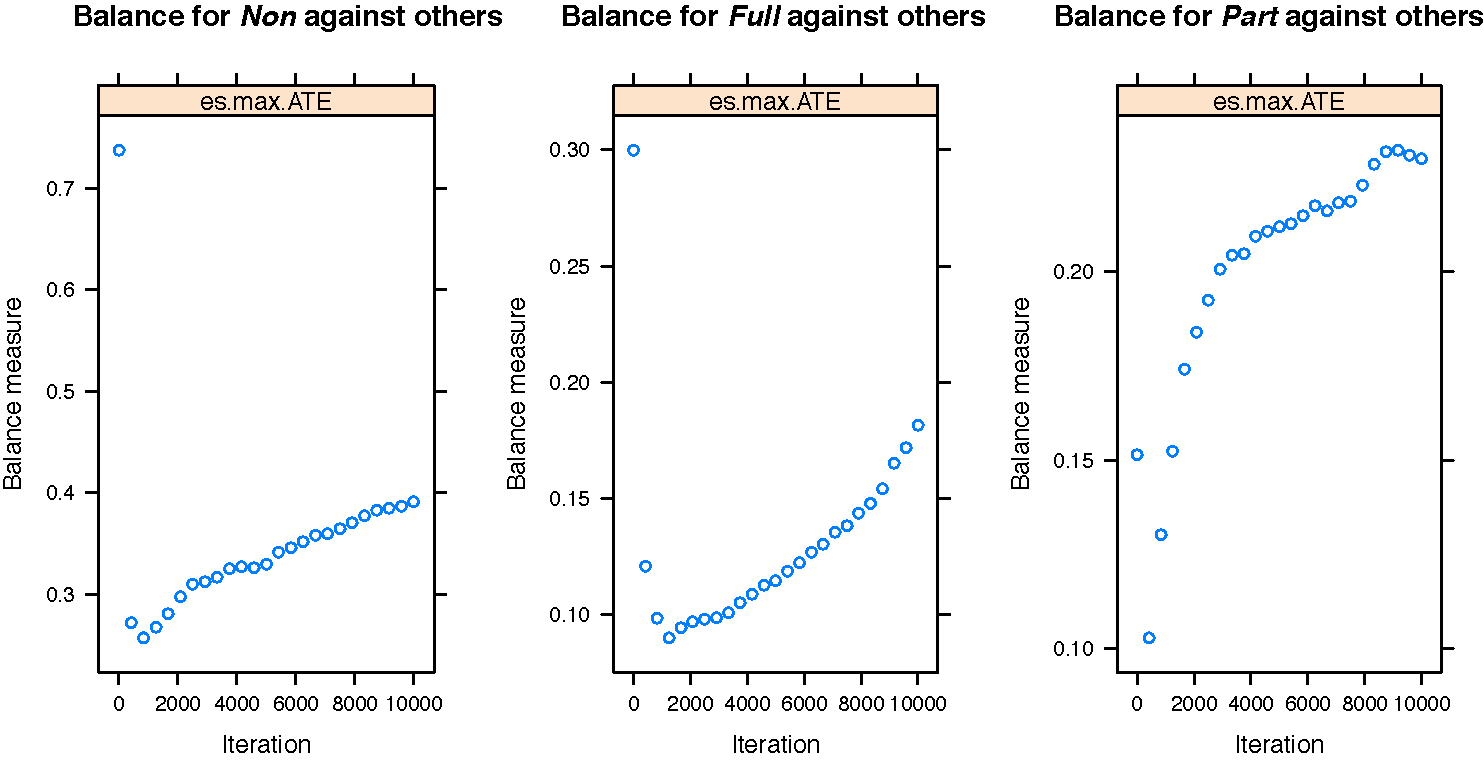
\includegraphics[width=\textwidth]{psdiag1.pdf}
\caption{{\bf GBM iterations and balance measure}}
\label{fig:diag1}
\end{center}
\end{figure}

\subsection{Overlapping assumption satisfied}
One key assumption of propensity score analysis is the overlapping assumption. Propensity score analyses assume that each experiment unit has a non-zero probability of receiving each treatment \citep{mnps2015}. We can examine the plausibility of this assumption by evaluating the overlap of the empirical propensity score distribution. As shown in the Figure \ref{fig:diag2}, although physicians who fully adopted EHR have higher possibility to be in this treatment group, the overlap assumption generally seems to be met for each treatment group. 

\begin{figure}[!htb]
\begin{center}
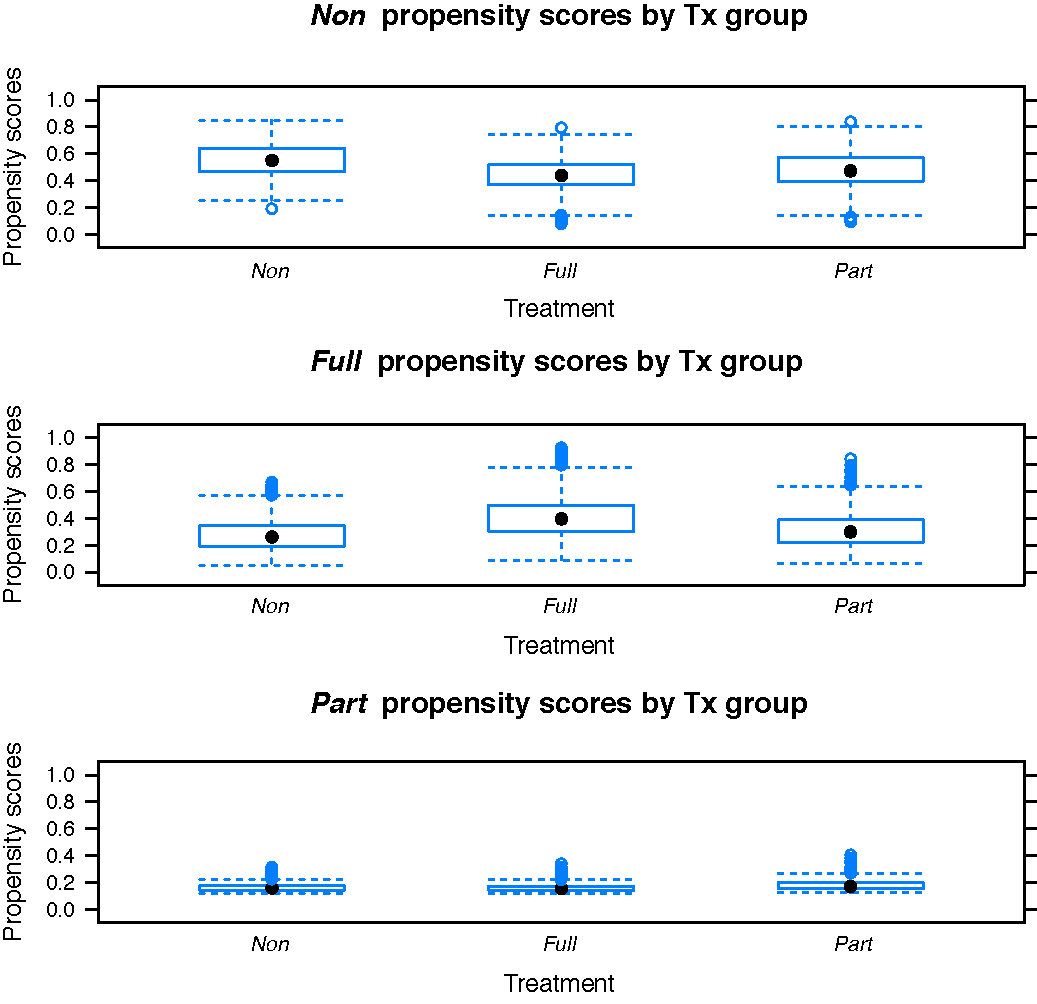
\includegraphics[width=\textwidth]{psdiag2.pdf}
\caption{{\bf Propensity score overlapping assumption}}
\label{fig:diag2}
\end{center}
\end{figure}

\subsection{Propensity score balance achieved}
Figure \ref{fig:diag3} and Figure \ref{fig:diag4} graphically summarize balance statistics from propensity score estimation with GBM model. In our analysis, each treatment variable of interest has three ASMD statistics, including the difference between non-adopter and fully adaptor, the difference between non-adopter and partially adopted and the difference between partially adopted and fully adopted. Figure \ref{fig:diag3} collapses these three statistics to covariate level and provides an overall comparison of the ASMD between each groups, before and after weighting. Figure \ref{fig:diag4} assesses the balance before and after weighting for each treatment group.The statistically significant difference is indicated by the solid circle.

As shown in the Figure \ref{fig:diag3}, covariates in unbalanced data is highly unbalanced. After weighting, the maximum ASMDs significantly decrease for highly unbalanced variables. Some well-balanced variables have slightly worse balances after weighting because those variables do not predict treatment, led to relatively random matching on them. As shown in the figure, the $ASMDs<0.25$ criterion is easily met for all pretreatment variables after propensity score weighting. Some variates have an ASMD greater than 0.1, which will be included in regression analysis later to achieve ``double robustness''.


\begin{figure}[!htb]
\begin{center}
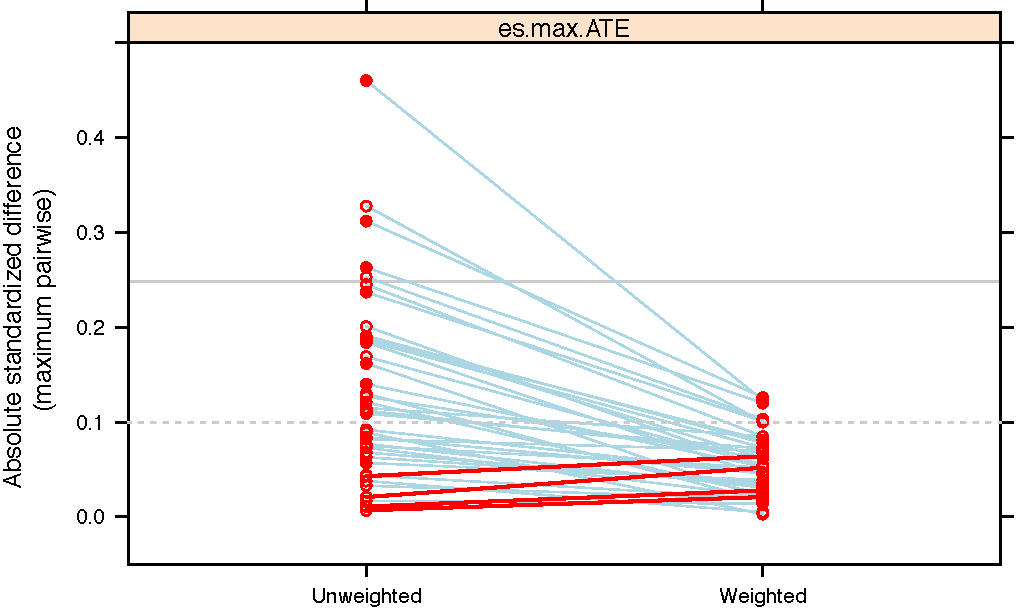
\includegraphics[width=\textwidth]{psdiag3.pdf}
\caption{{\bf Propensity score balancing}}
\label{fig:diag3}
\end{center}
\end{figure}

As shown in the Figure \ref{fig:diag4}, observed covariates are well-balanced between each possible pair of treatment in our analysis. Figure \ref{fig:diag4} illustrates the difference in maximum ASMDs by each treatment group before and after propensity score weighting. Physician practices in different treatment group have heterogeneous characterises before propensity score weighting procedure, especially between those who have fully adopted the EHR and those who have no EHR adoption (see left panel). Only one variable has not reached ASMD below 0.1 with statistical difference among all pairwise comparisons (see solid dot in weighted data, left panel). Although there are a few variables exceed 0.1 ASMD threshold in the middle and right penal, non of them are statistically significant. All variables in three treatment groups have less then 0.25 ASMD after propensity score weighting.

\begin{figure}[!htb]
\begin{center}
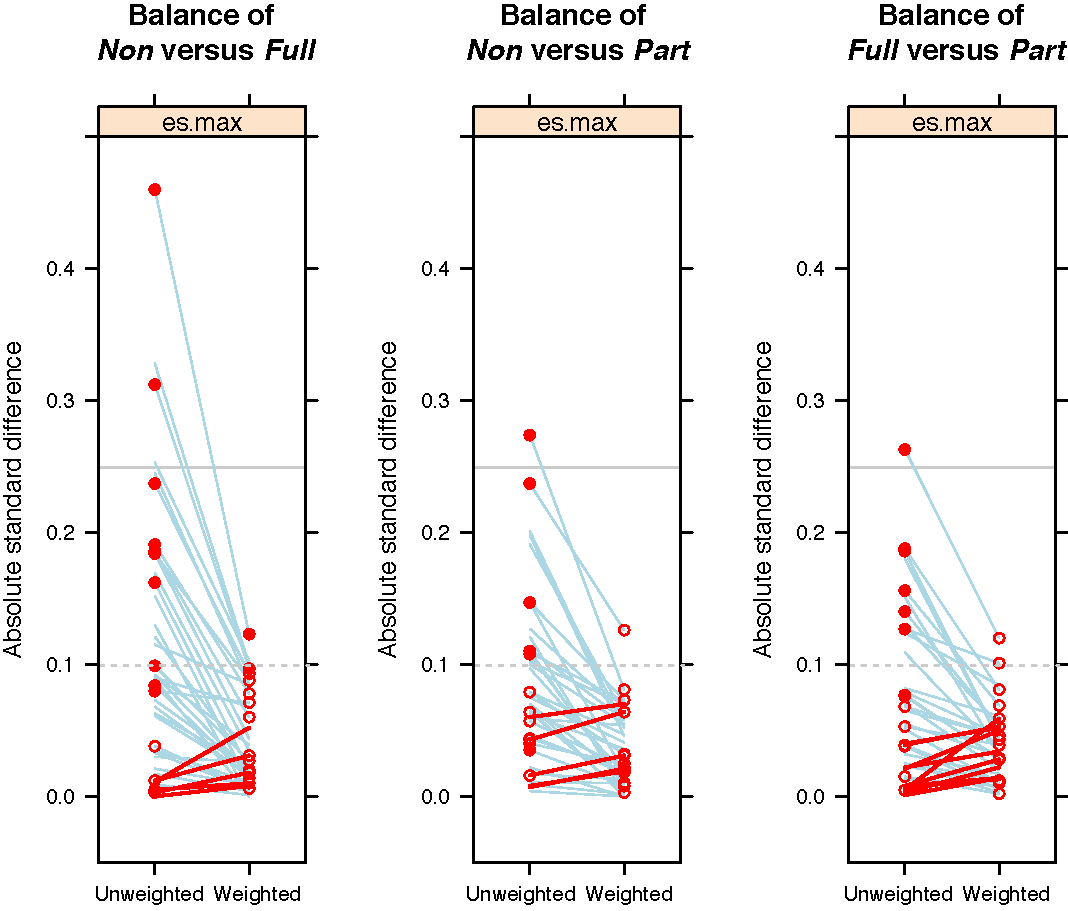
\includegraphics[width=\textwidth]{psdiag4.pdf}
\caption{{\bf Propensity score balancing by treatment group}}
\label{fig:diag4}
\end{center}
\end{figure}

\section{Tabular assessments of balance}
Table \ref{tab:ess} shows the effective sample size (ESS) before and after propensity score weighting. The ESS is approximately the number of observations from a simple random sample that yields an estimate with sampling variation equal to the sampling variation obtained with the weighted comparison observations \citep{twangvignettes}.  Overall, the effective has reduced to 60.86\% of sample without propensity score weighting. While this may seem like a large loss of sample size, this indicates that many of the physicians were observably unlike their counterparts in different treatment group and, hence, were not useful for isolating the treatment effect of the EHR system.

\begin{table}[h]
\caption{Effective sample size by treatment group}
\centering
\footnotesize
\label{tab:ess}
\begin{tabular}{lccc}
\hline \hline
Treatment & n    & ESS        & Proportion \\ \hline
Non       & 1853 & 1,116.9608 & 0.6028     \\
Full      & 1146 & 695.7736   & 0.6071     \\
Part      & 620  & 389.6171   & 0.6284     \\
          &     &               &           \\
All       & 3619 & 2,202.3515 & 0.6086     \\ \hline \hline 
\end{tabular}
\end{table}

Table \ref{tab:psbalance} shows maximum ASMDs of each covariates before and after propensity score weighting. Before propensity score weighting, the maximum ASMDs is 0.4605, which exceeds the 0.25 threshold and be considered as unacceptable. Only a few characteristics of physician practices are well-balanced with maximum ASMDs less than 0.1, including MSA status and average patient age, etc. The ownership type, physician specialities, solo status, and year of visit are highly unbalanced with maximum ASMDs greater than 0.25. 

The propensity score weighting procedure significantly improves the balance between each treatment groups. The maximum ASMDs in weighted sample is 0.1259, far below the 0.25 threshold. There are few variables have maximum ASMDs greater than 0.10 after weighting, including ownership type, managed care contracts, solo status, and visit year. MSA status, physician specialties, region, patient chronological conditions, physician age, and patient insurance type are considered as good balancing with ASMDs less than 0.1.



Although the observed covariates balanced relatively well, it is possible that unobserved differences between each two of three groups could still remain.


{\footnotesize
\begin{center}
\label{tab:psbalance}

\begin{longtable}{lcc}
\caption{Propensity Score Balance Statistics}\\

\hline \hline
Variable                               & \multicolumn{1}{p{3cm}}{\centering Max Std. ES \\(UNW)} & \multicolumn{1}{p{3cm}}{\centering Max Std. ES \\(PSW)} \\  \hline \endfirsthead

\caption*{Propensity Score Balance Statistics (Cont'd)}\\

\hline 
Variable                               & \multicolumn{1}{p{3cm}}{\centering Max Std. ES \\(UNW)} & \multicolumn{1}{p{3cm}}{\centering Max Std. ES \\(PSW)} \\  \hline \endhead

\hline  \multicolumn{3}{r}{\textit{table continues}}\\ \endfoot
\hline \hline  \textit{Note:} $^{*}$ Std. ES $>0.1000$ \endlastfoot


                                       &                          &                           \\
\textbf{Ownership Type}                &                          &                           \\
Physician or physician group           & 0.3123$^{***}$               & 0.1259$^{*}$                \\
Health Maintenance Organization (HMO)  & 0.2530$^{***}$               & 0.1033$^{*}$                \\
Community health center                & 0.1089$^{*}$               & 0.0725                    \\
Medical/academic health center         & 0.0680                   & 0.0337                    \\
Other hospital                         & 0.0754                   & 0.0524                    \\
Other health care corporation          & 0.1693$^{*}$               & 0.0549                    \\
Other                                  & 0.0922                   & 0.0470                    \\
                                       &                          &                           \\
\textbf{Metropolitan Statistical Area} &                          &                           \\
MSA                                    & 0.0427                   & 0.0643                    \\
Non-MSA                                & 0.0427                   & 0.0643                    \\
                                       &                          &                           \\
\textbf{Managed Care Contracts}        &                          &                           \\
None                                   & 0.2372$^{*}$               & 0.1006$^{*}$                \\
Less than 3                            & 0.0111                   & 0.0285                    \\
3-10                                   & 0.1209$^{*}$               & 0.0235                    \\
Greater than 10                        & 0.2452$^{*}$               & 0.0853                    \\
                                       &                          &                           \\
\textbf{Physician specialties}         &                          &                           \\
General/family practice                & 0.1913$^{*}$               & 0.0776                    \\
Internal medicine                      & 0.0818                   & 0.0702                    \\
Pediatrics                             & 0.0167                   & 0.0145                    \\
General surgery                        & 0.0893                   & 0.0032                    \\
Obstetrics and gynecology              & 0.0070                   & 0.0208                    \\
Orthopedic surgery                     & 0.0632                   & 0.0364                    \\
Cardiovascular diseases                & 0.2011$^{*}$               & 0.0520                    \\
Dermatology                            & 0.1907$^{*}$               & 0.0615                    \\
Urology                                & 0.0730                   & 0.0219                    \\
Psychiatry                             & 0.3280$^{***}$               & 0.0998                    \\
Neurology                              & 0.1297$^{*}$               & 0.0168                    \\
Ophthalmology                          & 0.1840$^{*}$               & 0.0435                    \\
Otolaryngology                         & 0.0384                   & 0.0048                    \\
Other specialties                      & 0.0206                   & 0.0516                    \\
Oncology                               & 0.1266$^{*}$               & 0.0624                    \\
                                       &                          &                           \\
\textbf{Solo}                                   & 0.4605$^{***}$               & 0.1233$^{*}$                \\
                                       &                          &                           \\
\textbf{Region}                        &                          &                           \\
Northeast                              & 0.0568                   & 0.0395                    \\
Midwest                                & 0.1122$^{*}$               & 0.0680                    \\
South                                  & 0.0331                   & 0.0191                    \\
West                                   & 0.1146$^{*}$               & 0.0850                    \\
                                       &                          &                           \\
\textbf{Avg. chron cond.}              & 0.1618$^{*}$               & 0.0199                    \\
\textbf{Avg. patient age}              & 0.0768                   & 0.0306                    \\
                                       &                          &                           \\
\textbf{Patient insurance type}        &                          &                           \\
Private insurance                      & 0.0837                   & 0.0457                    \\
Medicare                               & 0.1882$^{*}$               & 0.0815                    \\
Medicaid                               & 0.1398$^{*}$               & 0.0526                    \\
Workers Compensation                   & 0.0440                   & 0.0199                    \\
Self-pay                               & 0.1860$^{*}$               & 0.0727                    \\
                                       &                          &                           \\
\textbf{Visit Year}                    & 0.2630$^{***}$               & 0.1199$^{*}$    \\

\end{longtable}
\end{center}}

\chapter{Regression results}

% Table created by stargazer v.5.1 by Marek Hlavac, Harvard University. E-mail: hlavac at fas.harvard.edu
% Date and time: Tue, Mar 10, 2015 - 20:45:36
% Requires LaTeX packages: dcolumn 
\begin{table}[!htbp] \centering 
  \caption{Estimated effect of EMR adoption with multinomial 
          propensity score weighted OLS models} 
  \label{tab:mnps} 
\footnotesize 
\begin{tabular}{@{\extracolsep{5pt}}lD{.}{.}{-3} D{.}{.}{-3} D{.}{.}{-3} } 
\\[-1.8ex]\hline 
\hline \\[-1.8ex] 
 & \multicolumn{3}{c}{\textit{Dependent variable:}} \\ 
\cline{2-4} 
\\[-1.8ex] & \multicolumn{1}{c}{Health Edu.} & \multicolumn{1}{c}{Time Utilization} & \multicolumn{1}{c}{Ret. Appt. Rate} \\ 
\\[-1.8ex] & \multicolumn{1}{c}{(1)} & \multicolumn{1}{c}{(2)} & \multicolumn{1}{c}{(3)}\\ 
\hline \\[-1.8ex] 
 Full EMR & 0.034^{*} & 0.222 & -0.031^{**} \\ 
  & (0.018) & (0.532) & (0.015) \\ 
  Partial EMR & 0.033 & 0.189 & -0.008 \\ 
  & (0.020) & (0.574) & (0.018) \\ 
  SOLO & -0.007 & 2.158^{***} & 0.023 \\ 
  & (0.020) & (0.545) & (0.015) \\ 
  HMO$^a$ & 0.074^{*} & 0.647 & -0.142^{***} \\ 
  & (0.043) & (0.971) & (0.049) \\ 
  Community health center$^a$ & 0.007 & -3.222^{***} & 0.031 \\ 
  & (0.028) & (0.676) & (0.023) \\ 
  Medical/academic health center$^a$ & -0.015 & 3.993^{*} & 0.074^{*} \\ 
  & (0.049) & (2.081) & (0.040) \\ 
  Other hospital$^a$ & 0.037 & -1.920^{***} & 0.033 \\ 
  & (0.047) & (0.644) & (0.029) \\ 
  Other health care corporation$^a$ & 0.005 & 0.223 & -0.071^{**} \\ 
  & (0.035) & (0.775) & (0.030) \\ 
  Other owner type$^a$ & 0.029 & 3.438 & 0.030 \\ 
  & (0.050) & (2.094) & (0.052) \\ 
  MCC less than$^b$ 3 & -0.008 & -1.894 & 0.030 \\ 
  & (0.040) & (1.319) & (0.032) \\ 
  MCC 3-10$^b$ & -0.048 & -4.217^{***} & 0.020 \\ 
  & (0.032) & (1.119) & (0.028) \\ 
  MCC greater than 10$^b$ & -0.063^{**} & -5.571^{***} & 0.003 \\ 
  & (0.031) & (1.088) & (0.028) \\ 
  2009$^c$ & 0.033^{*} & -0.385 & 0.031^{*} \\ 
  & (0.019) & (0.528) & (0.016) \\ 
  2010$^c$ & 0.075^{***} & 0.576 & 0.033^{*} \\ 
  & (0.021) & (0.573) & (0.017) \\ 
  Constant & 0.411^{***} & 25.074^{***} & 0.679^{***} \\ 
  & (0.031) & (1.102) & (0.026) \\ 
 \hline \\[-1.8ex] 
Observations & \multicolumn{1}{c}{3,619} & \multicolumn{1}{c}{3,619} & \multicolumn{1}{c}{3,619} \\ 
Log Likelihood & \multicolumn{1}{c}{-2,048.801} & \multicolumn{1}{c}{-14,216.760} & \multicolumn{1}{c}{-1,394.416} \\ 
Akaike Inf. Crit. & \multicolumn{1}{c}{4,127.603} & \multicolumn{1}{c}{28,463.530} & \multicolumn{1}{c}{2,818.832} \\ 
\hline 
\hline \\[-1.8ex] 

  \multicolumn{4}{p{\textwidth}}{ \textit{Note: $^a$Comparing with physician or physician group. $^b$Comparing with practices with non managed care contracts. $^c$Comparing with year 2008. $^{*}$p$<$0.1; $^{**}$p$<$0.05; $^{***}$p$<$0.01}}\\
\end{tabular} 
\end{table} 

\chapter{Appendix}
\section{Sensitivity test results}



\newpage
\bibliographystyle{plainnat}
\bibliography{EHR}

\end{document}
